%# -*- coding: utf-8-unix -*-
%%==================================================
%% chapter01.tex for SJTU Master Thesis
%%==================================================

%\bibliographystyle{sjtu2}%[此处用于每章都生产参考文献]
\chapter{模型性能测试}
\label{chap:exper}



\section{数据集描述}

正确选择数据集是实验成功的关键,与模型要求相合的数据集可以助实验事半功倍。首先我们考虑了自己编写爬虫程序爬取数据的可能性,但是这种做法没办法取得标签信息,人工进行标签处理又是一件十分枯燥且主观成分浓厚的事情,这对于实验是没有好处的。经过讨论,我们还是选择了使用别人收集好的数据集。前人的工作中有很多已经整理好的数据集,而且各有特色。Jindal等人 \parencite{Jindal:2008}发布了一个亚马逊的评论数据集,但是亚马逊平台与我们模型的目标不合;Li等人 \parencite{Li:2014}与大众点评公司合作,发布了一个大众点评的数据集,但是这个数据集没有包含店铺的位置信息;Rayana等人 \parencite{Rayana:2015}发布了一个自己搜集的Yelp数据集,包含店铺的评论信息和Yelp过滤系统给这些评论打的标签,但是这个数据集中的评论是按照店铺归类的。还有很多其他的数据集,都与我们实验的设想有很大差异。

最后,我们找到了Santosh等人 \parencite{Santosh:2016}使用过的Yelp数据集。这是一个部分标签的数据集,包含店铺的地址信息,而且评论信息也按照评论账户做了归类,非常适合我们的模型。数据集的标签部分中,每一条评论都被Yelp的过滤系统分类为了“虚假评论”或“普通评论”。数据集的各类相关数据量如表~\ref{tbl:dataset}所示,数据集中一共含有760212条评论和16941组用户信息,其中带标签的评论有107624条,所有评论都被打过标签的用户有3142个。在107624条带标签评论中,20267条是虚假评论。这个数据集还有一个特色,那就是每一个被打过标签的用户的过滤比(即该用户所有评论中虚假评论的占比)都在0-20\%或90-100\%区间内。由于数据集本身并没有对用户进行标签处理,所以我们定义过滤比大于90\%的用户为水军用户,过滤比小于20\%的用户为普通用户。在这个分类标准下,3124个所有评论都被打过标签的用户中有1299个水军用户。此外,为了减少测试误差,一些发表评论数过低的用户将被过滤掉,不参与实际的计算。将评论数阈值设置为5的话,参与计算的用户数量将剩下11917个,所有评论都被打过标签的用户只剩下1796个。

\begin{table}[htbp]
	\caption[数据集相关数据]{数据集相关数据}
	\label{tbl:dataset}
	\centering
	\begin{tabular}{ccc}
		\toprule
		& 带标签的个数 & 总数  \\
		\midrule
		评论数  & 107624  & 760212  \\
		用户数  & 3142  &	16941 \\
		水军评论数 & 20267 & N/A \\
		水军用户数 & 1299 & N/A \\
		过滤后用户数 & 1796 & 11917 \\
		\bottomrule
	\end{tabular}
\end{table}

\section{实验描述}

本节我们将介绍实验的设置。模型使用的地理位置特征是通过经纬度计算出来的,店铺的经纬度是使用一个名为\emph{geocoder}的python库,利用其中的\emph{Arcgis}地图提供的地理位置编码功能从地址转换而来的。SpamTracer的模型参数是利用训练集训练得到的,测试是基于测试数据集的。训练集和测试数据集是数据集中包含标签部分内的不相交的两个集合。一个严重的问题是,数据集内的普通用户数据量和水军用户数据量是不平衡的,比例约为3:1,而实际上O2O平台的水军用户相比于普通用户也是占少数的那部分。在这样不平衡的数据集下,分类器需要能够抵挡数据的不平衡带来的影响。许多传统的分类算法在不平衡数据集中不能正常发挥,而SpamTracer可以经受大量误导数据的影响,准确地检测出小部分水军。

我们设计了对照组来测试SpamTracer的各项指标,这些对照组都是经典的分类方法。公平起见,我们选择的对照组都是监督型(Supervised)的算法,和SpamTracer的类型一致。对照组包含四个分类器:朴素贝叶斯NB、聚类算法AdaBoost、支持向量机SVM和多层感知机MLP(Multi-layer Perceptron)。这四个分类算法分别属于生成类模型、聚类模型、回归类模型和神经网络模型,可以作为机器学习领域中各类算法的经典代表。对照组的模型使用用户的账户相关特征作为检测依据,包括评论数量、账号的朋友数量、账号的粉丝数量、被选为优质评论的数量等。所有模型在测试中都使用10层交叉验证(Cross Validation)以保证测试结果的可靠性。


\section{模型测试结果}

参与模型测试的模型信息与测试结果如下:

\begin{enumerate}	
	\item[(1)] \textbf{SpamTracer}:本次毕业设计提出的SpamTracer模型
	\item[(2)] \textbf{NB}:朴素贝叶斯分类器
	\item[(3)] \textbf{AdaBoost}:AdaBoost分类器
	\item[(4)] \textbf{SVM-rbf}:以径向基函数rbf(Radial Basis Function)作为核函数的支持向量机模型
	\item[(5)] \textbf{MLP-relu}: 以线性整流函数relu(Rectified Linear Unit)作为激活函数的多层感知机模型
\end{enumerate}


\begin{figure}[htbp]
	\centering
	\begin{minipage}[htbp]{0.8\textwidth}
		\centering
		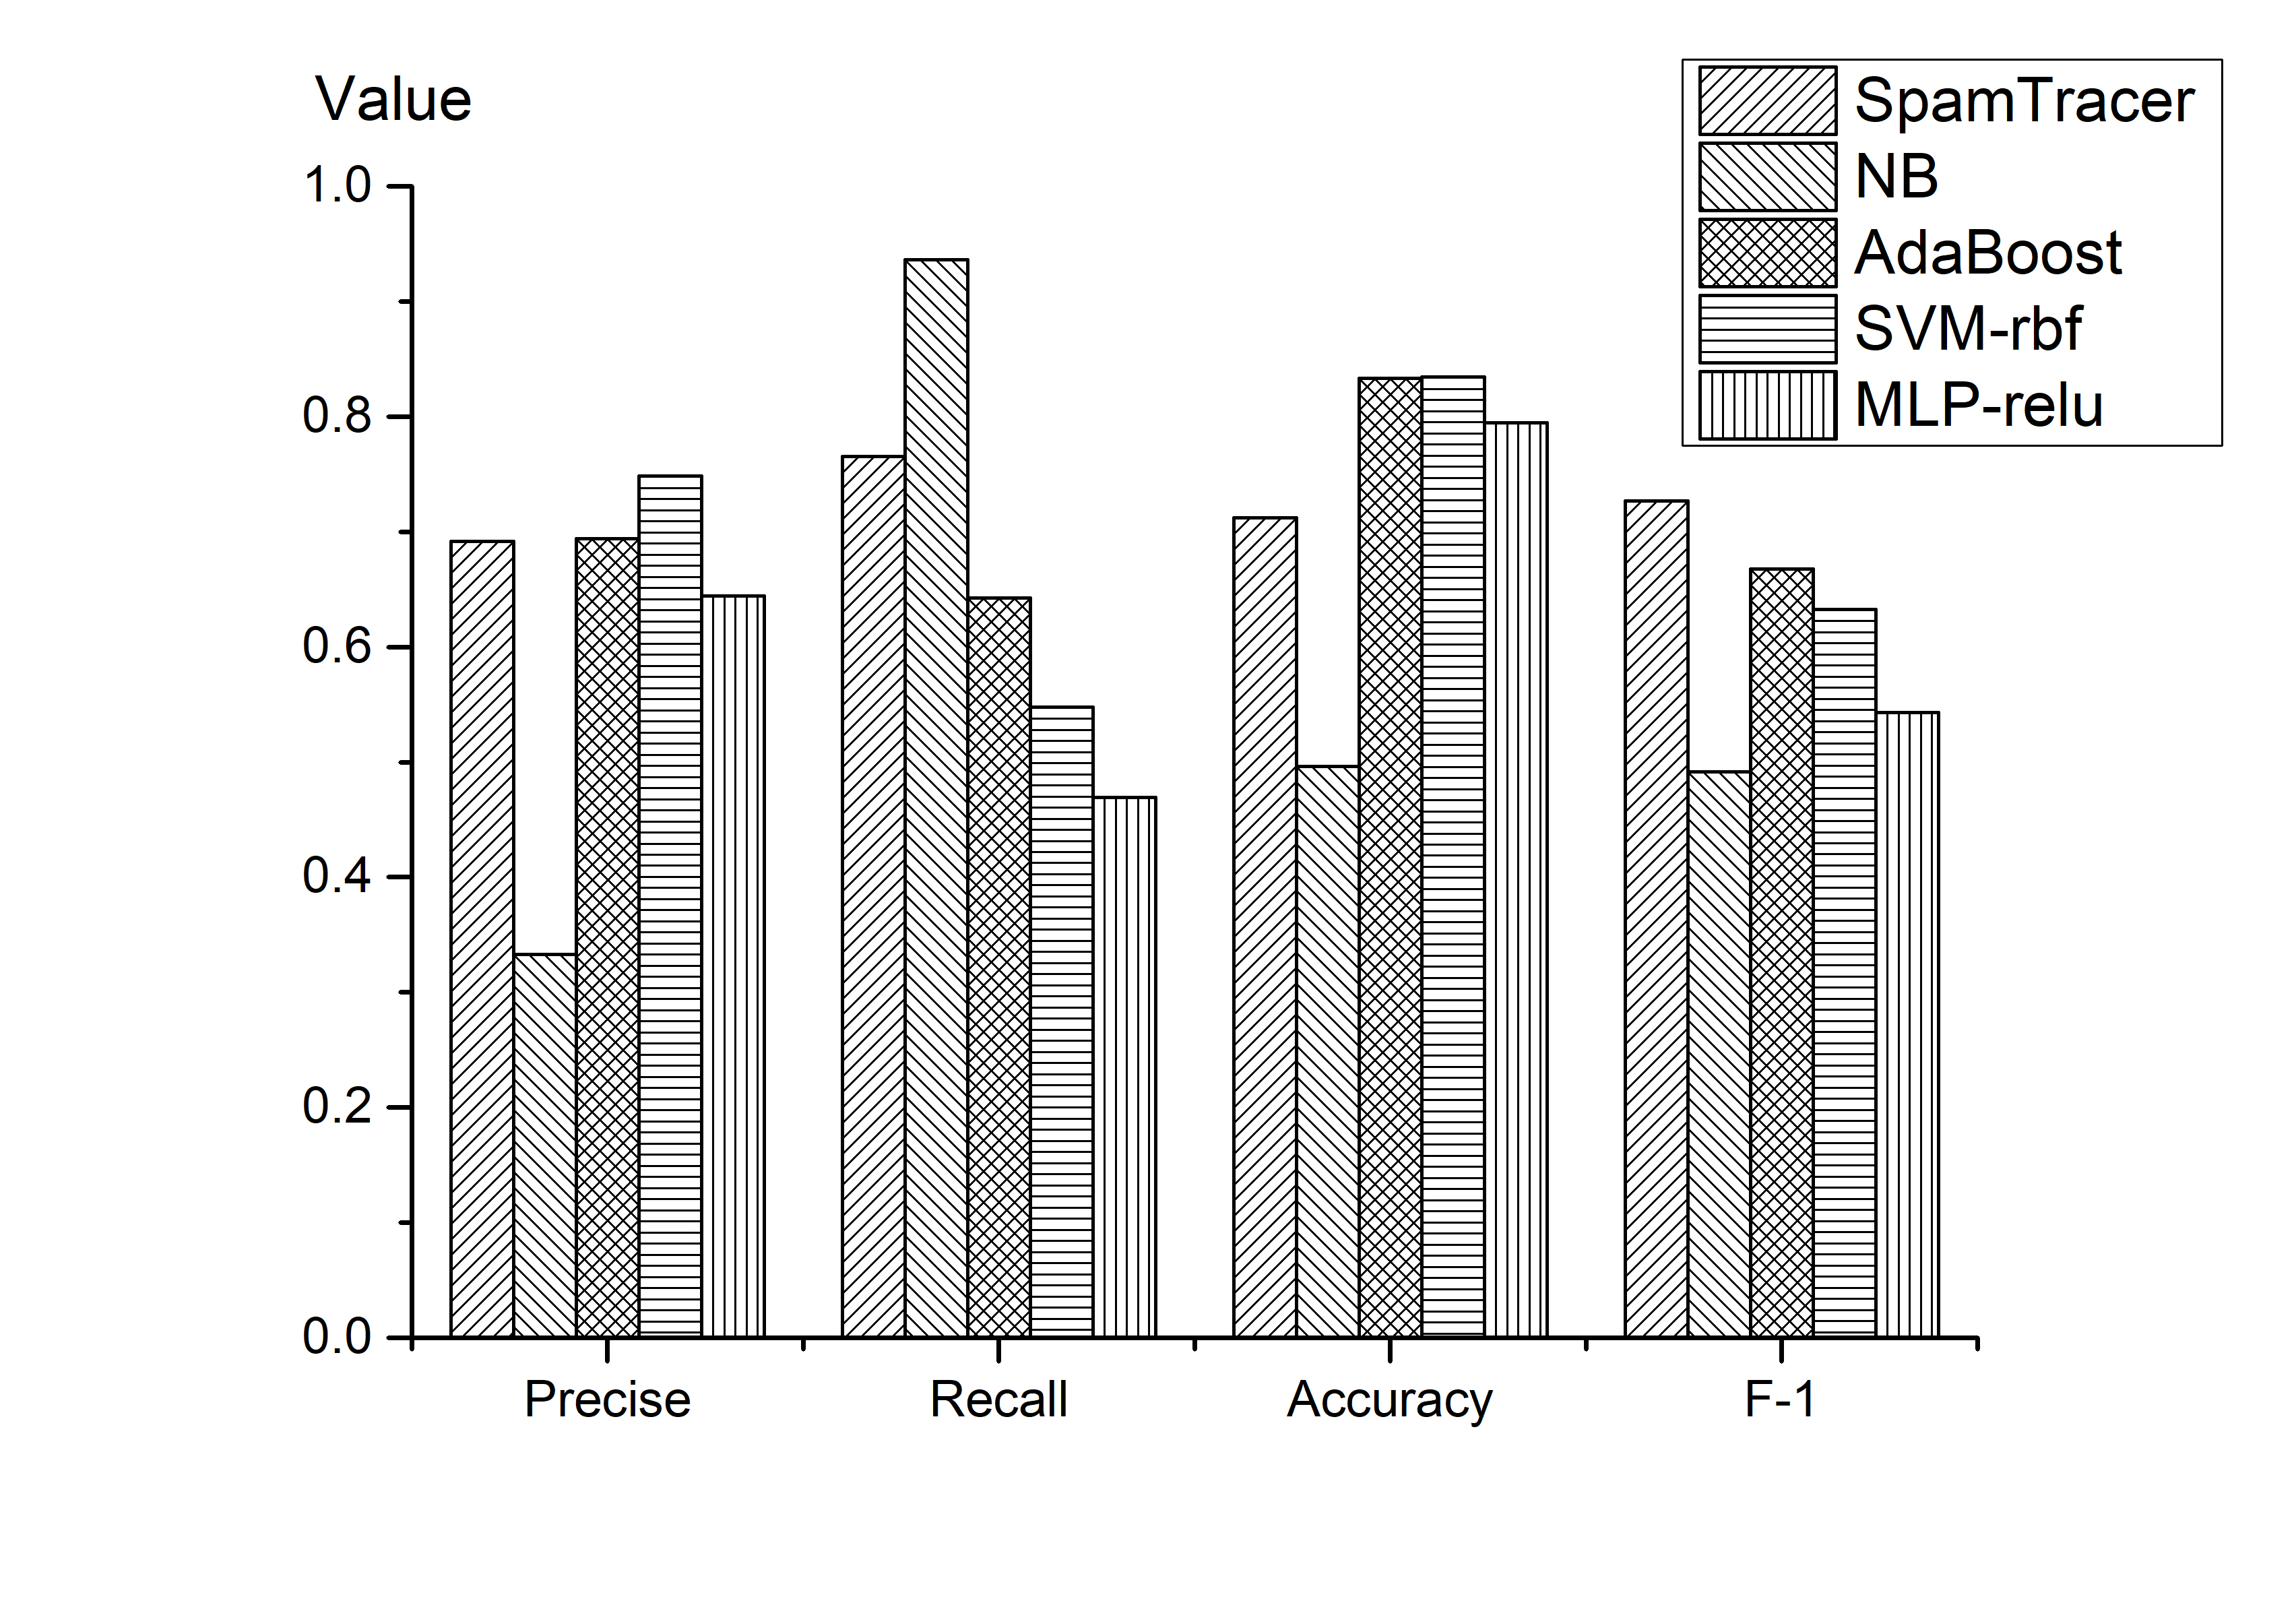
\includegraphics[width=10cm]{Result3.jpg}
		\caption[各模型的测试结果]
		{各模型的测试结果\label{fig:result}}		
	\end{minipage}     
\end{figure}


\begin{table}[htb]
	\centering
	\caption[各模型的精确度Precision、召回率Recall、准确率Accuracy和F1值]{各模型的精确度Precision、召回率Recall、准确率Accuracy和F1值}
	\label{tbl:Result}
	\begin{tabular}{ccccc}	
		\toprule
		& Precision & Recall & Accuracy & F1-score \\
		\midrule
		SpamTracer & 0.6917  & 0.7657 & 0.7122   &	0.7268 \\
		NB				& 0.3332  &	0.9365 & 0.4962   &	0.4916 \\
		AdaBoost		& 0.6945  &	0.6430 & 0.8336   &	0.6677 \\
		SVM-rbf			& 0.7484  &	0.5482 & 0.8346   &	0.6328 \\
		MLP-relu		& 0.6443  &	0.4694 & 0.7946   &	0.5431 \\
		\bottomrule
	\end{tabular}
\end{table}

我们对模型的评价基于四项广泛使用的评价标准:精确度(Precision)、召回率(Recall)、准确率(Accuracy)和F1值。图~\ref{fig:result}展示了上述五个模型在这四个方面的表现。SpamTracer模型在四个指标中的表现都很均衡,没有很突出的地方也没有明显的短板,是一个十分稳定可靠的模型;NB模型拥有最高的召回率,但是在其他三个指标上都是表现的最差的;AdaBoost模型和SVM-rbf模型的表现相对稳定,但是与SpamTracer相比还是浮动程度较大,而且在召回率上远远落后于SpamTracer;MLP-relu在精确度和准确率上表现较好,但是在召回率和F1上表现最差,也是一个表现不稳定的模型。综上所述,在我们的测试实验中SpamTracer在稳定性和准确度上都表现优秀。为了提供参考,表~\ref{tbl:Result}展示了图~\ref{fig:result}实验结果中的具体数字。此外,各个模型的测试结果在数值上都较低,我们认为这是来自不平衡数据集的影响。两类数据的数量差距悬殊,以及数据集的规模不是很大,对经典的分类算法们造成了较大冲击。

然而,我们也必须承认,SpamTracer的整体性能仍然有进步的空间。关于限制SpamTracer性能的因素,我们认为主要有两点:其一,SpamTracer的性能受到数据形式的影响较大。根据前文所述,SpamTracer具有链状结构,处理的数据形式是序列型的。而且根据前文的分析,数据序列的长度对模型的性能至关重要。序列长度越长,不同序列间的区分度就会越大,模型的分类性能越好。然而尽管我们已经做了过滤处理,忽略那些评论数过于少的用户,但数据集中数据序列的整体长度仍然不高,这会干扰模型的判断,导致准确率没有达到很高。其二,数据集的规模也是影响因素。如果我们能够获得规模更大的数据集,那么无论是在训练层面还是测试层面都会有巨大的性能提升。

总体来说,SpamTracer模型拥有优秀的稳定性,良好的准确率,并能在不平衡的数据集中有超出平均水平的表现。受到悬殊的数据量差距的冲击,经典模型们无法在各项指标中找到平衡点,表现极其不稳定。如果我们需要一个精确又稳定的模型作为O2O平台的过滤系统,那么SpamTracer将是一个既不会大量误伤普通用户,也不会放过大量可疑用户的好选择。


\section{水军行动规律验证}

本节我们将讨论第~\ref{chap:appli}章提出的利用SpamTracer模型验证水军行动规律的实验结果。使用SpamTracer扩展了数据集后,我们拥有694020条评论、228859家店铺、11058位用户以及包含在其中的4269位水军用户。所有的用户的评论都被打上了标签信息。数据集中搜集到的评论时间主要分布在2008年至2011年之间。该实验中,我们主要关注三类关系:水军数量与日期的关系,水军数量与开业时间的关系,以及共享水军数量与店铺距离间隔的关系。接下来我们将叙述我们在实验中的发现,并在图~\ref{fig:S}中展示一些可以支持我们实验结果的图像。

\begin{figure}[htp]
	\subcaptionbox{一年内的水军行动折线图\label{figure:s-a}} %标题的长度,超过则会换行,如下一个小图。
	{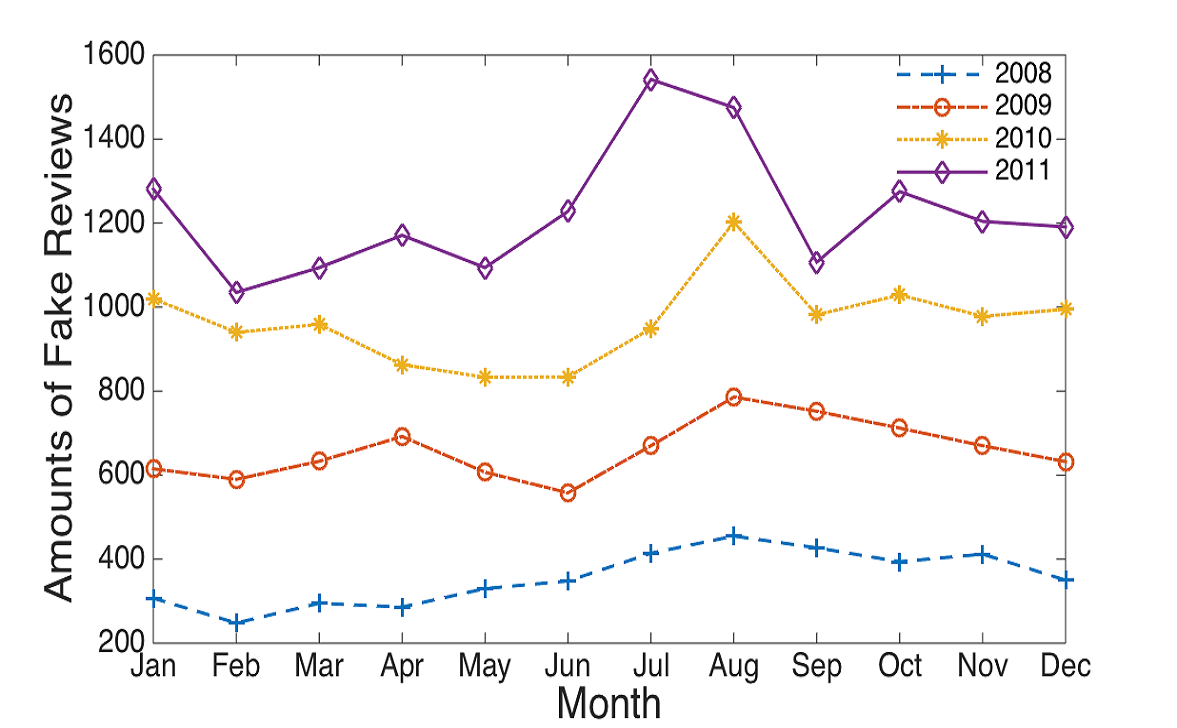
\includegraphics[height=4.5cm]{S1-Month.png}}
	\hspace{4em}
	\subcaptionbox{一周内的水军行动折线图\label{figure:s-b}}
	{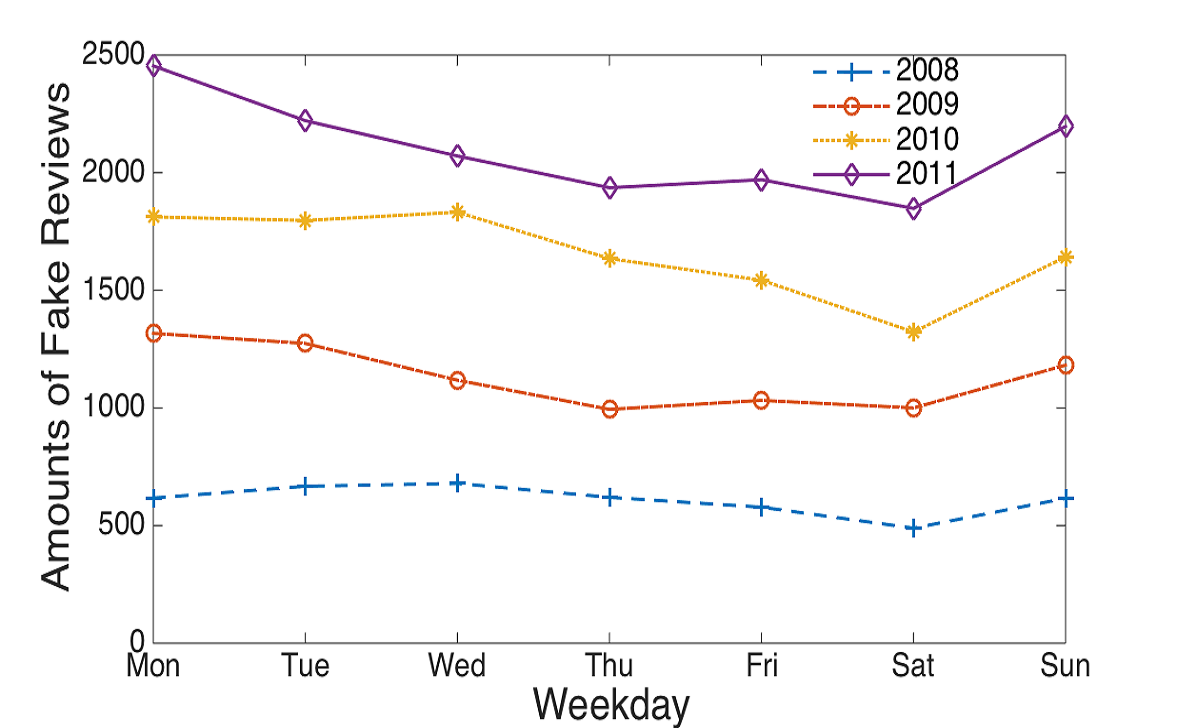
\includegraphics[height=4.5cm]{S1-Weekday.png}}
	\hspace{4em}
	\subcaptionbox{开业时间与水军数量关系图\label{figure:s-c}}
	{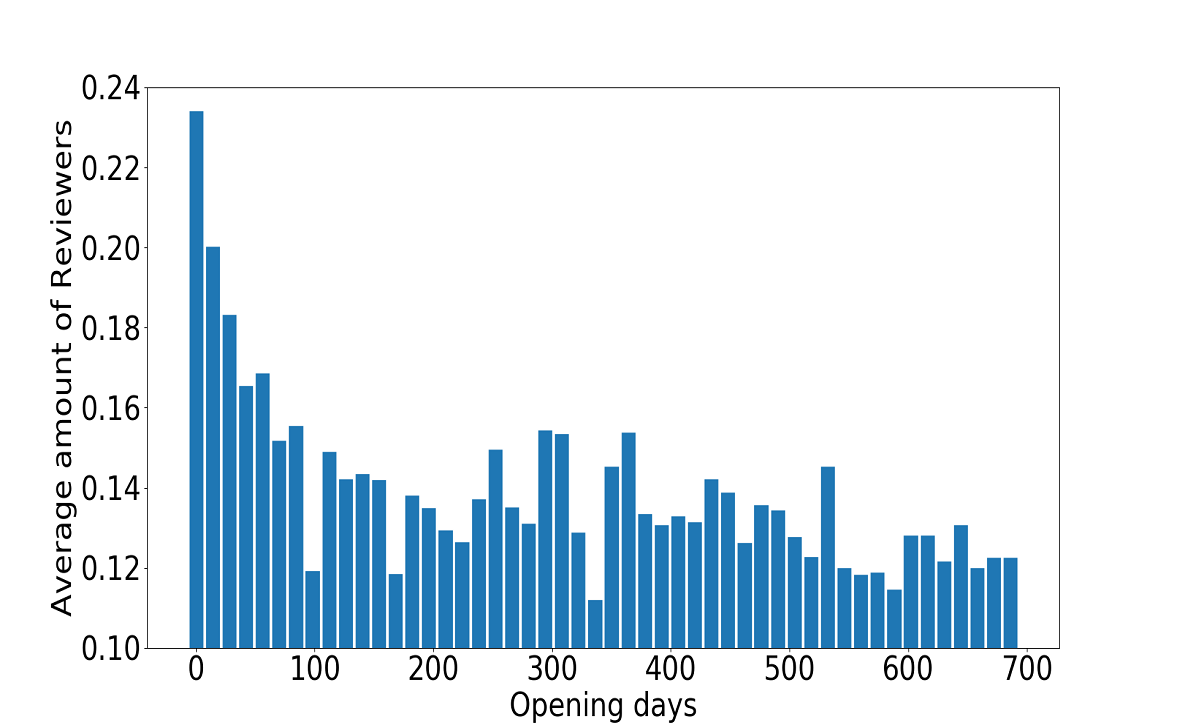
\includegraphics[height=4.5cm]{S2-Amount.png}}
	\hspace{4em}
	\subcaptionbox{店铺数量与水军评论占比关系图\label{figure:s-d}}
	{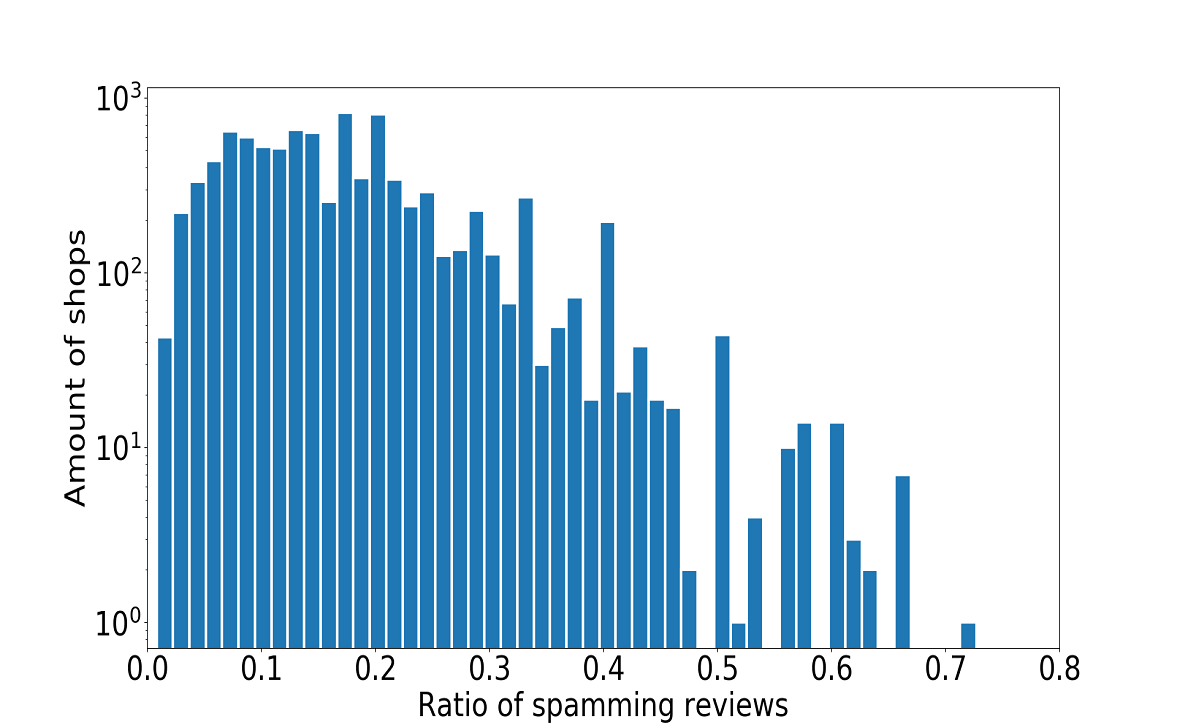
\includegraphics[height=4.5cm]{S2-Ratio-1.png}}
	\hspace{4em}
	\subcaptionbox{共有水军数量与店铺间距关系图\label{figure:s-e}}
	{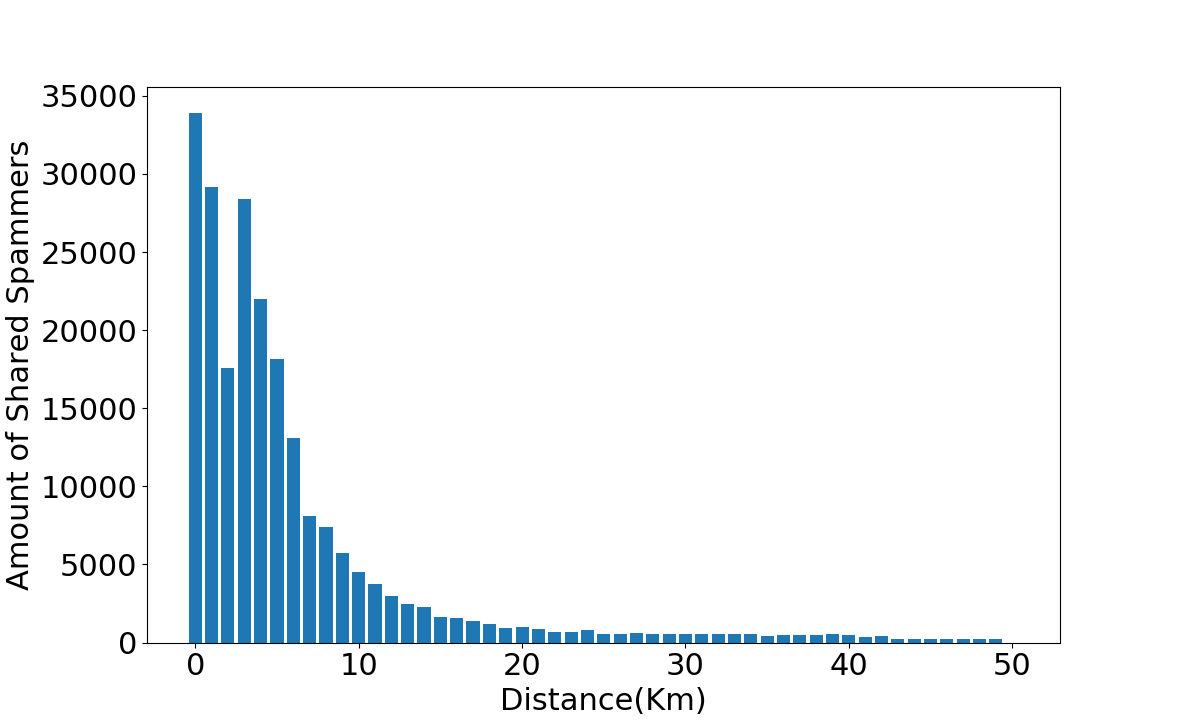
\includegraphics[height=4.5cm]{S3-Amount-1.png}}
	\hspace{4em}
	\subcaptionbox{共有水军比例与店铺间距关系图\label{figure:s-f}}
	{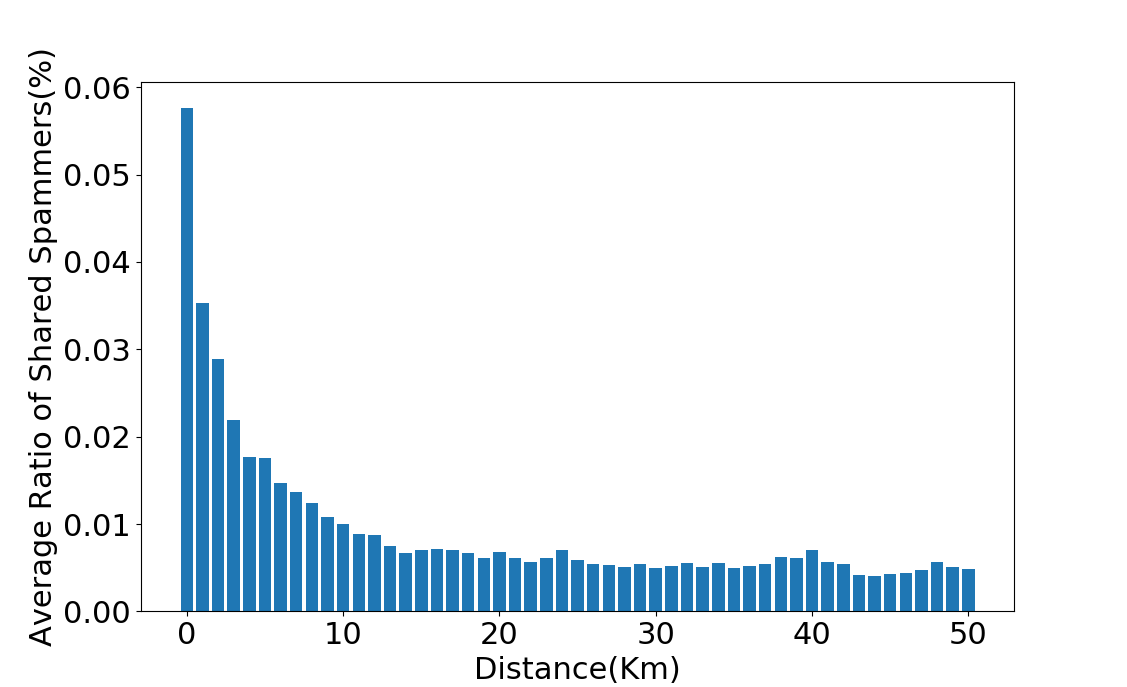
\includegraphics[height=4.5cm]{S3-Ratio-1.png}}
	\caption[水军行动规律验证]{水军行动规律验证}
	\label{fig:S}
\end{figure}

\subsection{水军数量与日期}

水军们倾向于在每年的夏季进行频繁的水军行动,以及在每周的周日和周一进行频繁的水军活动。我们提取了数据集中收集的水军评论的发布时间,并按照月份和按照一星期内的每天进行归类。图~\ref{figure:s-a}和图~\ref{figure:s-b}分别展示了2008年至2011年间水军行动在月份和星期内每天上的分布情况。图~\ref{figure:s-a}的横坐标表示月份,纵坐标表示虚假评论数量,显示出一年内的各个季节中夏季的水军评论数量显著高于其他季节的水军评论数量。我们认为这个现象与旅游相关。美国国家旅游办公室NTTO(National Travel \& Tourism Office)\footnote{https://travel.trade.gov/research/monthly/arrivals/index.asp}的数据显示,每年第三季度(七月、八月和九月)来访的海外游客数量是全年中最多的。庞大的客流量刺激店铺们雇佣更多的水军宣传他们的店铺以获得更多游客的青睐。此外,图~\ref{figure:s-b}的横坐标表示一星期内的不同日子,纵坐标表示虚假评论数量,显示了水军们倾向于在每周的周日和周一进行水军活动。这个结论也与我们的认知相吻合。在此之外,我们发现两幅折线图反映出了一个客观现象:水军评论的数量在逐年增长。2008年的水军评论有67705条,而到了2011年水军评论数量激增到了140722条。这也从侧面反映出了近年来水军产业的快速发展。



\subsection{水军数量与开业时间}

与经验结论相同,在店铺开业初期出现的水军评论数量最多。在我们的实验中,为了避免无效的数据影响结果,我们排除了那些开业时间不足一年的店铺,以及评论数少于五条的店铺。过滤后剩余21000家店铺,关于它们的开业时间与每日水军数量的关系图如图~\ref{figure:s-c}所示。横坐标代表店铺的开业时间,纵坐标代表每家店铺的平均水军数量。关系图显示店铺的开业初期出现了更多的水军,然后随着时间增加,店铺平均水军数量逐渐减少。此外,我们还绘制了反映店铺的评论中水军评论比例与店铺数量的关系图,如图~\ref{figure:s-d}。图~\ref{figure:s-d}的横坐标是店铺的所有评论中的水军评论占比,纵坐标是水军评论占比在该区间内的店铺数量。这幅图显示相当比例店铺雇佣过水军,甚至还有一些店铺的半数以上评论都是虚假评论,印证了“店铺雇佣水军来自我宣传”这一潜规则的真实性。


\subsection{共有水军数量与店铺的间隔距离}

我们发现两个店铺的共有水军数量与这两个店铺的间距成反比例关系。然而,这样的共有水军仅仅占了总水军的很小的比例。根据第~\ref{chap:appli}章提出的算法,我们设计了实验。实验中我们设置店铺评论数过滤阈值为2,过滤后的店铺数量是102478。共有水军数量与店铺间距的关系,以及共有水军比例与店铺间距的图像分别如图~\ref{figure:s-e}和图~\ref{figure:s-f}所示。图~\ref{figure:s-e}的横坐标为店铺间距离,纵坐标为共有水军数量,图~\ref{figure:s-f}的横坐标为店铺间距离,纵坐标为共有水军数量占总水军数量的比例。图像显示了共有水军的确存在,而且与店铺间距呈反比例关系。然而,图~\ref{figure:s-f}显示共有水军在全部水军中的占比非常低,当店铺间距接近0时,共有水军占比最高也只有0.06\%,而随着距离增加,共有水军比例减少,最后逐渐稳定在0.006\%左右。根据两幅图得出的结论是:水军同时与商圈内复数家店铺进行合作的现象的确存在,但是这并不是水军行动的主流现象,不必投入过多关注。



